\chapter{Console I/O}
IO stands for input/output. C provides only mechanism to interact through
console using its standard library. C does not provide ways to have GUI
although that is possible with various GUI libraries most notable being
GTK. However, discussing about GTK is out of scope of this book. In this
chapter we will focus on console output facilities of C because any program we
write at this stage will be meaningless if it has no input/output. Typically
when we interact with a C program we give input using keyboard which is also
referred as \texttt{stdin} stream. The output is monitor or \texttt{stdout}
stream. There is one more stream \texttt{stderr} which is generally redirected
to monitor or a log file. For historical reasons these are known as
\texttt{FILE} stream which represents the datatype of these
streams. \texttt{FILE} is capable of representing other streams which are disk
based for example a file on your hard drive. There are more type of input
devices on a modern computer. For example, network i/o is there. Whenever you
browse web or download a file through your intenet connection network i/o comes
into play. There is an opengroup
which specifies functions for network related functions. Operating systems
like GNU/Linux are POSIX compatible which defines how network i/o will be
used. Even a printer is a special output device, a camera input, speakers
output, microphone input and so on. In this books we are concerned with
keyboard input, output on monitor and i/o using files. Other types of i/os are
out of scope of this book.

However, before we go on with i/o I would
like to present C's memory model which will be needed by our discussion of i/o
related functions. However, if things do not make sense even then please go
through it and come later to understand more. 

\section{C's Memory Model}
As you may be knowing RAM(random acess memory) is the area which is used as
primary memory. Whenever we execute a program the first thing which happens is
that it gets loaded into memory. Now a binary program becomes a process when it
is running i.e. a running program is referred as process. All processes have
memory area divided into different portions. These portions are known as data
segment, stack and code or text segment. Dats segement is further split in
three parts; initialized data segment, uninitialized data segment or BSS which
is name after an ancient assembler Block Started by Symbol and
heap. Initialized data segment contains initialized global variables and static
variables. For uninitialized data segment it is same as above just that the
variables are not initialized explicitly but implicitly to zero.

Heap is the largest area of memory used for dynamic memory allocation. As
you will see later that you can manage heap using \texttt{malloc(), calloc(),
realloc(),} and \texttt{free()}. Note that compiler does not manage memory
allocated for you. You, the programmer, are responsible for allocating and
freeing up memory in area. If heap gets full os will use virtual memory or swap
space on hard disk. Objects allocated on heap persist across function
calls. However, there are some very nasty problems, which, come in picture when
you use heap. There are several of them. You may forget to allocate memory and
want to dereference unallocated pointer. You may have initialized it to
\texttt{NULL} and try to dereference that. You may allocate and free twice. You
forgot to set pointer to \texttt{NULL} after freeing it. And last but not the
least you loose all pointers to the memory area before you can free. The nature
with this particular problem is that if your program is going to run for long
time then it is going to consume more and more memory. Because of its nature it
is known as memory leak. It is very difficult to detect such problems in code
which does not run for long periods of time. Our friend valgrind will come to
help up with this problem. When a memory leak happens it eats up RAM slowly and
then operating system has to use virtual memory as explained above. In a
nutshell, I will say that heap means you have to manage it.

\begin{figure}[t!]
\begin{center}
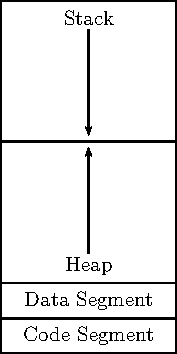
\includegraphics{figs/mem_model.pdf}
\end{center}
\caption{Memory model of a C program}
\end{figure}

Stack is relatively simple. All non-static and non-register variables go on
stack. Stack variables do not retain there value across function calls unless
they are passed as pointers or static variables. Also, when they go out of
scope, that is the scope in which they were declared ends, they will be kind of
lost. The way in which stack frame moves the same area will be used for new
variables. However, stack is very limited (compared to heap) and in deeply
nested function calls or recursion (you will see these in Functions chapter)
stack may get full and program may crash. The reason for crashing is that
operating system will not use virtual memory but will do a segmentation fault
in its place. GNU/Linux allow its users to modify the stack size by ulimit
command. Note that stack and heap are adjacent in memory and grow in opposite
direction.

Code segment or text segment is an area where the executable instructions of
program reside. It is typically constant and read-only area unless your system
allows self-modifying code. Following diagram shows the memory layout.

Note that this memory model not only applies to C but any process.

Now we will look at those functions, which, allow us to do console i/o. We will
begin with our familiar friends; printf and scanf.

\section{printf}
The prototype of \texttt{printf} is given by

\begin{minted}{c}
int printf(const char* fmt, ...);
\end{minted}

Let us take a minute to understand this as we have not yet covered
functions. The first word is \texttt{int} which denotes the return type of the
\texttt{printf} function. This is no. of characters printed. Then we have name
of the function. \texttt{fmt} is the format string of type \texttt{const
 char}. In C, strings are either character arrays or character pointers. Here,
const means \texttt{printf} will not modify the format string. The ... means
variable no. of arguments, which, can be 0 also to be supplied to
\texttt{printf}.

\texttt{printf} is a string based output function that is It writes character
strings to \texttt{stdout}. The data which has to be written is formatted by
format string as shown previously. After the format specifier it expects as
many arguments as specified in format string. The characters which are not
like, say \texttt{\%d} for example, arecalled ordinary characters. These are
simply copied to output stream, which, is stdout for printf. The \texttt{\%d}
like conversion charcaters are known as conversion specification or format
specifiers. Each conversion specification should be augmented with one one
argument. The results are undefined if there are insufficient arguments for the
format. If extra arguments are given the excess arguments will be evaluated but
are otherwise ignored. However, there is a big problem here! There is no
type-safety. In general compiler will warn you about it and you, the
programmer, are responsible for giving correct format string, correct no. of
correct type of arguments. Consider the following program for example:

\begin{minted}{c}
#include <stdio.h>

int main()
{
  printf("%d %d\n", 3, 8);

  //do not mess it. undefined behavior
  printf("%d %d\n", 5);

  //extra arguments ignored
  printf("%d %d\n", 3, 5, "hello");

  //legal because char is integer type
  printf("%d\n", 's');

  //wrap around of integer as char
  printf("%c\n", 836);

  //do not mess with type-safety
  int i = printf("%d\n", "hello");
  prinf("%d\n", i);

  return 0;
}
\end{minted}

now that if you give the command like \texttt{gcc -Wall printf.c} where
\texttt{printf.c} is the name of the ile then you will be shown following
warnings:

\begin{verbatim}
printf.c: In function 'main':
printf.c:8:3: warning: format '%d' expects a matching 'int' argument [-Wformat=]
   printf("%d %d\n", 5);
   ^
printf.c:8:3: warning: format '%d' expects a matching 'int' argument [-Wformat=]
printf.c:11:3: warning: too many arguments for format [-Wformat-extra-args]
   printf("%d %d\n", 3, 5, "hello");
   ^
printf.c:11:3: warning: too many arguments for format [-Wformat-extra-args]
printf.c:20:3: warning: format '%d' expects argument of type 'int', but
argument 2 has type 'char *' [-Wformat=]
   int i = printf("%d\n", "hello");
   ^
printf.c:20:3: warning: format '%d' expects argument of type 'int', but
argument 2 has type 'char *' [-Wformat=]
\end{verbatim}

Clearly this is not a good sign for any program. A program should compile
cleanly. In our case \texttt{gcc} is generating binary even though there are
warnings. You can make \texttt{gcc} generate more warnings by issuing a
\texttt{-Wall} flag. You can also treat all warnings as errors by passing
\texttt{-Werror} to \texttt{gcc}. These two options will ensure that your code
has no warnings. Now let us move to output and try to understand it. The output
on my system is as given below. It may differ on your system:

\begin{verbatim}
3 8
5 8
3 5
115
D
134514119
10
\end{verbatim}

First \texttt{printf} is correct as expected. The second line causes undefined
behavior. You may think it is the previous 8 but believe me it is not
guaranteed that it will always the case. Ii is \textbf{UNDEFINED}. Third
\texttt{printf} is also fine in the sense that extra argument is
ignored. Fourth and fifth are normal. Sixth is again a big problem. You are
trying to print a decimal integer while argument is a character string. There
is no way for compiler to determine that what should be printed which will fit
on standards. Now we will have to take a look at all possible format specifier
and their meanings. You have seen most of them so this is more for a
reference. Once again the following is taken from specification for
correctness. Do not worry if you do not understand all of it now as it will all
become clear in due course of time. Just make sure you read it carefully.

\section{Conversion Specification}
Each conversion specification starts with \texttt{`\%'} character. After this
following appear in sequence:

\begin{itemize}
\item[---] Zero or more flags, in any order, which modify the meaning of the
  conversion specification. 
\item[---] An optional minimum field width. If the converted value from argument has
  fewer characters (bytes) than the field width, it will be padded with spaces
  by default on left; it will be padded on right if the left-adjustment flag
  ('-') is given to the field width. The field width takes the form of an
  asterisk or a decimal integer. 
\item[---] An optional precision that gives the minimum number of digits to appear
  for the \texttt{d, i, o, u, x} and \texttt{X} conversion specifiers; the
  number of digits to appear for radix character for the \texttt{a, A, e, E, f}
  and \texttt{F} conversion specifiers; the maximum number of significant
  digits for the \texttt{g} and \texttt{G} conversion specifiers; or the
  maximum number of bytes to be printed from a string in the \texttt{s}
  conversion specifiers. The precision takes form of a period (`.') followed
  either by an asterisk (`*'), described below, or an optional decimal digit
  string, where a null digit string is treated as zero. If a precision appears
  with any other conversion specifier, the behavior is undefined.
\item[---] An optional length modifier that specifies the size of the argument.
\item[---] A conversion specifier character that indicates the type of conversion
  to be applied. 
\end{itemize}

A field width, or precision, or both, may be indicated by an asterisk(`*'). In
this case an argument of type int supplies the field width or precision. You,
the programmer, will have to ensure that arguments specifying field, width or
precision, or both appear in that order before the argument, if any to be
converted. A negative field width is taken as a `-' flag followed a positive
field width. A negative precision is taken as if the precision were omitted.

The flag characters and their meanings are:

\begin{longtable}{m{0.1\textwidth}m{0.85\textwidth}}
\textbf{-}&The result of the conversion will be left-justified within the field. The
conversion is right-justified if the flag is not specified.\\
\textbf{+}&The result of a signed conversion will always begin with a sign (`+'
or `-'). The conversion will begin with a sign only when a negative value is
converted if this value is not specified.\\
\textit{space}&If the first character of a signed conversion is not a sign or if a signed
conversion results in no characters, a will be prefixed to the result. This
means that if the and `+' flags both appear, the flag will be ignored.\\
\textbf{\#}& Specifies that the value is to be converted to an alternative
form. For \texttt{o} conversion, it increases the precision (if necessary) to
force the first digit of the result to be zero. For \texttt{x} or \texttt{X}
conversion specifiers, a non-zero result will have \texttt{0x (0X)} prefixed to
it. For \texttt{a, A, e, E, f, F, g} and \texttt{G} conversion specifiers, the
result will always contain a radix character, even if no digits follow the
radix character. Without this flag, a radix character appears in the result of
these conversions only if a digit follows it.
For \texttt{0} and \texttt{G} conversion specifiers, trailing zeros will not be
removed from the result as they normally are. For other conversion specifiers
the, the behavior is \textbf{UNDEFINED}.\\
\textbf{0}&For \texttt{d, i, o, x, X, a, A, e, E, f, F, g} and \texttt{G}
conversion specifiers, leading zeros (following any indication of sign or base)
are used to pad to the field width; no space padding is performed. If the `0'
and `-' flags both appear, the `0' flag is ignored. For \texttt{d, i, o, u, x}
and \texttt{X} conversion specifiers, if a precision is specified, the `0' flag
is ignored.
\end{longtable}

The length and their meanings are:

\begin{longtable}{m{0.1\textwidth}m{0.85\textwidth}}
\textbf{hh}&Specifies that a following \texttt{d, i, o, u, x} and \texttt{X}
conversion specifiers applies to a \texttt{signed char} or \texttt{unsigned
  char} argument (the argument will have been promoted according to integer
promotions, but its value will be converted to) \texttt{signed char} or
\texttt{unsigned char} before printing; or that a following n conversion
specifier applies to a pointer to a \texttt{signed char} argument.\\
\textbf{h}&Specifies that a following \texttt{d, i, o, u, x} and \texttt{X}
conversion specifier applies to a \texttt{short} or \texttt{unsigned short}
argument (the argument will have been promoted according to the integer
promotions, but its value will be converted to \texttt{short} or
\texttt{unsigned short} before printing); or that a following n conversion
specifier applies to a pointer to a \texttt{short} argument.\\
\textbf{l}&Specifies that a following \texttt{d, i, o, u, x} and \texttt{X}
conversion specifier applies to a \texttt{long} or \texttt{unsigned long}
argument; that a following \texttt{n} conversion specifier applies to a pointer
to a \texttt{long} argument; that a following \texttt{c} conversion specifier
applies to a \texttt{win\_t} argument; that a following \texttt{s} conversion
specifier applies to a \texttt{wchat\_t} argument; or has not effect on a
following \texttt{a, A, e, R, f, F, g} or \texttt{G} conversion specifier.\\
\textbf{ll}&Specifies that a following \texttt{d, i, o, u, x} and \texttt{X}
conversion specifier applies to a \texttt{long long} or \texttt{unsigned long
  long} argument; that a following \texttt{n} conversion specifier applies to a
pointer to a \texttt{long long} argument.\\
\textbf{j}&Specifies that a following \texttt{d, i, o, u, x} and \texttt{X}
conversion specifier applies to an \texttt{intmax\_t} or \texttt{uintmax\_t}
argument; or that a following \texttt{n} conversion specifier applies to an
\texttt{intmax\_t} argument.\\
\textbf{z}&Specifies that a following \texttt{d, i, o, u, x} and \texttt{X}
conversion specifier applies to a \texttt{size\_t} or the corresponding signed
integer type argument; or that a following n conversion specifier applies to a
signed integer type corresponding to a \texttt{size\_t} argument.\\
\textbf{t}&Specifies that a following \texttt{d, i, o, u, x} and \texttt{X}
conversion specifier applies to a \texttt{ptrdiff\_t} or the corresponding
\texttt{unsigned int} type argument; or that a following \texttt{n} conversion
specifier applies to a \texttt{unsigned int} type corresponding to a
\texttt{ptrdiff\_t} argument.\\
\texttt{L}&Specifies that a following \texttt{a, A, e, E, f, F, g} or
\texttt{G} conversion specifier applies to a \texttt{long double} argument.
\end{longtable}

If a length modifier appears with any conversion specifier other than as
specified above, the behavior is undefined.

The conversion specifiers and their meanings are:

\begin{longtable}{p{0.1\textwidth}p{0.85\textwidth}}
\texttt{d, i}&The int argument is converted to signed decimal in the style
\textit{[-]dddd}. The precision specifies the minimum number of digits to
appear; if the value being converted can be represented in fewer digits, it is
expanded with leading zeros. The default precision is 1. The result of
converting a zero value with a precision of zero is no characters.\\
\texttt{o, u, x, X}&The \texttt{unsigned int} argument is converted to unsigned
octal (\texttt{o}), unsigned decimal (\texttt{u}), or unsigned hexadecimal
notation (\texttt{x} or \texttt{X}) in the style \textit{dddd}; the 
letters \texttt{abcdef} are used for \texttt{x} conversion and the letters
\texttt{ABCDEF} for \texttt{X} conversion. The precision specifies the minimum
number of digits to appear; if the value being converted can be represented in
fewer digits, it is expanded with leading zeros. The default precision is
1. The result of converting a zero value with a precision of zero is no
characters.\\
\texttt{f, F}&A \texttt{double} argument representing a floating-point number
is converted to decimal notation in the style \textit{[-]ddd.ddd}, where the
number of digits after the decimal-point character is equal to the precision
specification. If the precision is missing, it is taken as 6; if the precision
is zero and the \texttt{\#} flag is not specified, no decimal-point character
appears. If a decimal-point character appears, at least one digit appears
before it. The value is rounded to the appropriate number of digits.

A \texttt{double} argument representing an infinity is converted in one of the styles
\textit{[-]}\texttt{inf} or \textit{[-]}\texttt{infinity} --- which style is
implementation-defined. A double argument representing a NaN is converted in
one of the styles \textit{[-]}\texttt{nan} or
\textit{[-]}\texttt{nan}(n-char-sequence) --- which style, and the meaning of
any n-char-sequence, is implementation-defined. The \texttt{F} conversion specifier 
produces \texttt{INF, INFINITY} or \texttt{NAN} instead of \texttt{inf,
  infinity} or \texttt{nan} respectively.\footnote{When applied to infinite and
  NaN values, the \texttt{-, +} and \textit{space} flag characters have their
  usual meaning; the \texttt{\#} and \texttt{0} flag characters have no
  effect.}\\
\texttt{e, E}&A \texttt{double} argument representing a floating-point number
is converted in the style \textit{[-]d.ddd} \texttt{e}$\pm$\textit{dd}, where
there is one digit (which is nonzero if the argument is nonzero) before the
decimal-point character and the number of digits after it is equal to the
precision; if the precision is missing, it is 
taken as 6; if the precision is zero and the \texttt{\#} flag is not specified,
no decimal-point character appears. The value is rounded to the appropriate
number of digits. The \texttt{E} conversion specifier produces a number with
\texttt{E} instead of \texttt{e} introducing the exponent. The exponent always
contains at least two digits, and only as many more digits as necessary to
represent the exponent. If the value is zero, the exponent is zero.

A \texttt{double} argument representing an infinity or NaN is converted in the
style of an \texttt{f} or \texttt{F} conversion specifier.\\
\texttt{g, G}&A \texttt{double} argument representing a floating-point number
is converted in style \texttt{f} or \texttt{e} (or in style \texttt{F} or
\texttt{E} in the case of a \texttt{G} conversion specifier), depending on the
value converted and the precision. Let $P$ equal the 
precision if nonzero, 6 if the precision is omitted, or 1 if the precision is zero.
Then, if a conversion with style \texttt{E} would have an exponent of
$X$:
\begin{itemize}
\item[---] if $P > X \ge - 4$, the conversion is with style \texttt{f} (or
  \texttt{F}) and precision $P - (X + 1)$.
\item[---] otherwise, the conversion is with style \texttt{e} (or \texttt{E})
  and precision $P - 1$.
\end{itemize}
Finally, unless the \texttt{\#} flag is used, any trailing zeros are removed from the
fractional portion of the result and the decimal-point character is removed if
there is no fractional portion remaining.

A \texttt{double} argument representing an infinity or NaN is converted in the style
of an \texttt{f} or \texttt{F} conversion specifier.\\
\texttt{a, A}&A \texttt{double} argument representing a floating-point number
is converted in the style \textit{[-]}\texttt{0x}\textit{h.hhhh}
\texttt{p}$\pm$\textit{d}, where there is one hexadecimal digit (which is 
nonzero if the argument is a normalized floating-point number and is
otherwise unspecified) before the decimal-point character\footnote{Binary
  implementations can choose the hexadecimal digit to the left of the
  decimal-point character so that subsequent digits align to nibble (4-bit)
  boundaries.} and the number of hexadecimal digits after it is equal to the
precision; if the precision is missing and \texttt{FLT\_RADIX} is a power of 2,
then the precision is sufficient for an exact representation of the value; if
the precision is missing and \texttt{FLT\_RADIX} is not a power of 2, then the
precision is sufficient to distinguish\footnote{The precision $p$ is sufficient
  to distinguish values of the source type if $16^{p-1} > b^n$ where $b$ is 
\texttt{FLT\_RADIX} and $n$ is the number of base-$b$ digits in the significand
of the source type. A smaller $p$ might suffice depending on the
implementation's scheme for determining the digit to the left of the 
decimal-point character.} values of type \texttt{double}, except that trailing
zeros may be omitted; if the precision is zero and the \texttt{\#} flag is not
specified, no decimal-point character appears. The letters \texttt{abcdef} are
used for \texttt{a} conversion and the letters \texttt{ABCDEF} for \texttt{A}
conversion. The \texttt{A} conversion specifier produces a number with
\texttt{X} and \texttt{P} instead of \texttt{x} and \texttt{p}. The exponent
always contains at least one digit, and only as many more digits as necessary
to represent the decimal exponent of 2. If the value is zero, the exponent is
zero.

A \texttt{double} argument representing an infinity or NaN is converted in the
style of an \texttt{f} or \texttt{F} conversion specifier.\\
\texttt{c}&If no \texttt{l} length modifier is present, the \texttt{int}
argument is converted to an \texttt{unsigned char}, and the resulting character
is written.

If an \texttt{l} length modifier is present, the \texttt{wint\_t} argument is
converted as if by an \texttt{ls} conversion specification with no precision
and an argument that points to the initial element of a two-element array of
\texttt{wchar\_t}, the first element containing the \texttt{wint\_t} argument
to the \texttt{lc} conversion specification and the second a null wide
character.\\
\texttt{s}&If no \texttt{l} length modifier is present, the argument shall be a
pointer to the initial element of an array of character type.\footnote{No
  special provisions are made for multibyte characters.} Characters from the
array are written up to (but not including) the terminating null character. If
the precision is specified, no more than that many bytes are written. If the
precision is not specified or is greater than the size of the array, the array
shall contain a null character.

If an \texttt{l} length modifier is present, the argument shall be a pointer to
the initial element of an array of \texttt{wchar\_t} type. Wide characters from
the array are converted to multibyte characters (each as if by a call to the
\texttt{wcrtomb} function, with the conversion state described by an
\texttt{mbstate\_t} object initialized to zero before the first wide character
is converted) up to and including a terminating null wide character. The
resulting multibyte characters are written up to (but not including) the
terminating null character (byte). If no precision is specified, the array
shall contain a null wide character. If a precision is specified, no more than
that many bytes are written (including shift sequences, if any), and the array
shall contain a null wide character if, to equal the multibyte character
sequence length given by the precision, the function would need to access a
wide character one past the end of the array. In no case is a partial multibyte
character written.\footnote{Redundant shift sequences may result if multibyte
  characters have a state-dependent encoding.}\\
\texttt{p}&The argument shall be a pointer to \texttt{void}. The value of the
pointer is converted to a sequence of printing characters, in an
implementation-defined manner.\\
\texttt{n}&The argument shall be a pointer to signed integer into which is
\textit{written} the number of characters written to the output stream so far
by this call to \texttt{printf}. No argument is converted, but one is
consumed. If the conversion specification includes any flags, a field width, or
a precision, the behavior is undefined.
\texttt{\%} A \texttt{\%} character is written. No argument is converted. The
complete conversion specification shall be \texttt{\%\%}.
\end{longtable}

If a conversion specification is invalid, the behavior is undefined. If any
argument is not the correct type for the corresponding conversion
specification, the behavior is undefined.

In no case does a nonexistent or small field width cause truncation of a field;
if the result of a conversion is wider than the field width, the field is
expanded to contain the conversion result.

For \texttt{a} and \texttt{A} conversions, if \texttt{FLT\_RADIX} is a power of
2, the value is correctly rounded to a hexadecimal floating number with the
given precision.

In real-world most of the time the conversion specifiers are kept simple. Given
below is a sample program showing some of the things given above:

\begin{minted}{c}
#include<stdio.h>

int main()
{
  int i   = 343456;
  float f = 123;
  long double ld = 78939.9347;

  printf("% d\n", i);
  printf("%+d\n", i);
  printf("%#o\n", i);
  printf("%#f\n", f);
  printf("%-08i\n", i);
  printf("%08i\n", i);
  printf("%8i\n", i);
  printf("%hhi\n", i);
  printf("%hi\n", i);
  printf("%li\n", i);
  printf("%lli\n", i);
  printf("%ji\n", i);
  printf("%zi\n", i);
  printf("%ti\n", i);
  printf("%8.8f\n", f);
  printf("%8.8Lf\n", ld);

  return 0;
}
\end{minted}

The output of the above program is:

\begin{verbatim}
 343456
+343456
01236640
123.000000
343456
00343456
  343456
-96
15776
343456
4638355772471066016
4638355772471066016
343456
343456
123.00000000
78939.93470000
\end{verbatim}

We will keep seeing more conversion specifiers being used as we progress
through this book.

\section{scanf}
It scans \texttt{stdin} or keyboard for input. Its signature is same as that of
\texttt{printf()}. It reads bytes from keyboard input, interprets them
according to format string. It also expects a set of pointer arguments as
opposed to values for printf(). The pointers indicate where the interpreted
data from the input will be stored. The result is \texttt{UNDEFINED} if there
are less number of pointer arguments than the number of conversion specifers in
format string. Excess arguments will be evaluated but ignored. The format
string can have only white-space characters or an ordinary character (neither
`\%' nor a white-space character) or a conversion specification. Each
conversion specification is introduced by `\%', after which the following
appear in sequence.

For now if you do not understand what is a pointer then let us have a simple
definition for that. A pointer is a variable which stores a memory location
where the value will be stored. Once again following description is taken from
specification for correctness and completeness.

\begin{itemize}
\item[---] An optional assignment-suppressing character *.
\item[---] An optional decimal integer greater than zero that specifies the
  maximum field width (in characters).
\item[---] An optional \textit{length modifier} that specifies the size of the
  receiving object. 
\item[---] A \textit{conversion specifier} character that specifies the type of
  conversion to be applied.
\end{itemize}

The \texttt{scanf} function executes each directive of the format in turn. When
all directives have been executed, or if a directive fails (as detailed below),
the function returns. Failures are described as input failures (due to the
occurrence of an encoding error or the unavailability of input characters), or
matching failures (due to inappropriate input).

A directive composed of white-space character(s) is executed by reading input
up to the first non-white-space character (which remains unread), or until no
more characters can be read. The directive nev er fails.

A directive that is an ordinary multibyte character is executed by reading the
next characters of the stream. If any of those characters differ from the ones
composing the directive, the directive fails and the differing and subsequent
characters remain unread. Similarly, if end-of-file, an encoding error, or a
read error prevents a character from being read, the directive fails.

A directive that is a conversion specification defines a set of matching input
sequences, as described below for each specifier. A conversion specification is
executed in the following steps:

Input white-space characters (as specified by the \texttt{isspace} function)
are skipped, unless the specification includes a \texttt{[, c} or \texttt{n}
specifier.\footnote{These white-space characters are not counted against a
  specified field width.}

An input item is read from the stream, unless the specification includes an n
specifier. An input item is defined as the longest sequence of input characters
which does not exceed any specified field width and which is, or is a prefix
of, a matching input sequence.\footnote{\texttt{scanf} pushes back at most one
  input character onto the input stream. Therefore, some sequences that are
  acceptable to \texttt{strtod, strtol} etc., are unacceptable to
  \texttt{fscanf}.}The first character, if any, after the input item remains
unread. If the length of the input item is zero, the execution of the directive
fails; this condition is a matching failure unless end-of-file, an encoding
error, or a read error prevented input from the stream, in which case it is an
input failure.

Except in the case of a \% specifier, the input item (or, in the case of a
\texttt{\%n} directive, the count of input characters) is converted to a type
appropriate to the conversion specifier. If the input item is not a matching
sequence, the execution of the directive fails: this condition is a matching
failure. Unless assignment suppression was indicated by a *, the result of the
conversion is placed in the object pointed to by the first argument following
the \texttt{format} argument that has not already received a conversion
result. If this object does not have an appropriate type, or if the result of
the conversion cannot be represented in the object, the behavior is undefined.

The length modifiers and their meanings are:

\begin{longtable}{p{0.1\textwidth}p{0.85\textwidth}}
\texttt{hh}&Specifies that a following \texttt{d, i, o, u, x, X} or \texttt{n}
conversion specifier applies to an argument with type pointer to \texttt{signed
  char} or \texttt{unsigned char}.\\
\texttt{h}&Specifies that a following \texttt{d, i, o, u, x, X} or \texttt{n}
conversion specifier applies to an argument with type pointer to \texttt{short
  int} or \texttt{unsigned short int}.\\
\texttt{l} (ell)&Specifies that a following \texttt{d, i, o, u, x, X} or
\texttt{n} conversion specifier applies to an argument with type pointer to
\texttt{long int} or \texttt{unsigned long int}; that a following \texttt{a, A,
  e, E, f, F, g} or \texttt{G} conversion specifier applies to an argument with
type pointer to \texttt{double}; or that a following \texttt{c, s} or
\texttt{[} conversion specifier applies to an argument with type pointer to
\texttt{wchar\_t}.\\
\texttt{ll} (ell-ell)&Specifies that a following \texttt{d, i, o, u, x, X} or
\texttt{n} conversion specifier applies to an argument with type pointer to
\texttt{long long int} or \texttt{unsigned long long int}.\\
\texttt{j}&Specifies that a following \texttt{d, i, o, u, x, X} or \texttt{n}
conversion specifier applies to an argument with type pointer to
\texttt{intmax\_t} or \texttt{uintmax\_t}.\\
\texttt{z}&Specifies that a following \texttt{d, i, o, u, x, X} or \texttt{n}
conversion specifier applies to an argument with type pointer to
\texttt{size\_t} or the corresponding signed integer type.\\
\texttt{t}&Specifies that a following \texttt{d, i, o, u, x, X} or \texttt{n}
conversion specifier applies to an argument with type pointer to
\texttt{ptrdiff\_t} or the corresponding unsigned integer type.\\
\texttt{L}&Specifies that a following \texttt{a, A, e, E, f, F, g} or
\texttt{G} conversion specifier applies to an argument with type pointer to
\texttt{long double}.
\end{longtable}

If a length modifier appears with any conversion specifier other than as
specified above, the behavior is undefined.

The conversion specifiers and their meanings are:

\begin{longtable}{p{0.1\textwidth}p{0.85\textwidth}}
\texttt{d}&Matches an optionally signed decimal integer, whose format is the
same as expected for the subject sequence of the \texttt{strtol} function with
the value 10 for the \texttt{base} argument. The corresponding argument shall
be a pointer to signed integer.\\
\texttt{i}&Matches an optionally signed integer, whose format is the same as
expected for the subject sequence of the \texttt{strtol} function with the
value 0 for the \texttt{base} argument. The corresponding argument shall be a
pointer to signed integer.\\
\texttt{o}&Matches an optionally signed octal integer, whose format is the same
as expected for the subject sequence of the \texttt{strtoul} function with the
value 8 for the \texttt{base} argument. The corresponding argument shall be a
pointer to unsigned integer.\\
\texttt{u}&Matches an optionally signed decimal integer, whose format is the
same as expected for the subject sequence of the \texttt{strtoul} function with
the value 10 for the base argument. The corresponding argument shall be a
pointer to unsigned integer.\\
\texttt{x}&Matches an optionally signed hexadecimal integer, whose format is
the same as expected for the subject sequence of the \texttt{strtoul} function
with the value 16 for the base argument. The corresponding argument shall be a
pointer to unsigned integer.\\
\texttt{a, e, f, g}&Matches an optionally signed floating-point number,
infinity, or NaN, whose format is the same as expected for the subject sequence
of the \texttt{strtod} function. The corresponding argument shall be a pointer
to floating.\\
\texttt{c}&Matches a sequence of characters of exactly the number specified by
the field width (1 if no field width is present in the
directive).\footnote{\label{note1}No special provisions are made for multibyte
  characters in the matching rules used by the \texttt{c, s} and \texttt{[}
  conversion specifiers -- the extent of the input field is determined on a
  byte-by-byte basis. The resulting field is nevertheless a sequence of
  multibyte characters that begins in the initial shift state.}

If no \texttt{l} length modifier is present, the corresponding argument shall
be a pointer to the initial element of a character array large enough to accept
the sequence. No null character is added.

If an \texttt{l} length modifier is present, the input shall be a sequence of
multibyte characters that begins in the initial shift state. Each multibyte
character in the sequence is converted to a wide character as if by a call to
the \texttt{mbrtowc} function, with the conversion state described by an
\texttt{mbstate\_t} object initialized to zero before the first multibyte
character is converted. The corresponding argument shall be a pointer to the
initial element of an array of \texttt{wchar\_t} large enough to accept the
resulting sequence of wide characters. No null wide character is added.\\
\texttt{s}&Matches a sequence of non-white-space
characters.\footnotemark[\value{footnote}]

If no \texttt{l} length modifier is present, the corresponding argument shall
be a pointer to the initial element of a character array large enough to accept
the sequence and a terminating null character, which will be added
automatically.

If an \texttt{l} length modifier is present, the input shall be a sequence of
multibyte characters that begins in the initial shift state. Each multibyte
character is converted to a wide character as if by a call to the mbrtowc
function, with the conversion state described by an \texttt{mbstate\_t} object
initialized to zero before the first multibyte character is converted. The
corresponding argument shall be a pointer to the initial element of an array of
\texttt{wchar\_t} large enough to accept the sequence and the terminating null
wide character, which will be added automatically.\\
\texttt{[}&Matches a nonempty sequence of characters from a set of expected
characters (the \textit{scanset})\footnotemark[\value{footnote}].\\
&If no \texttt{l} length modifier is present, the corresponding argument shall
be a pointer to the initial element of a character array large enough to accept
the sequence and a terminating null character, which will be added
automatically.\\
&If an \texttt{l} length modifier is present, the input shall be a sequence of
multibyte characters that begins in the initial shift state. Each multibyte
character is converted to a wide character as if by a call to the
\texttt{mbrtowc} function, with the conversion state described by an
\texttt{mbstate\_t} object initialized to zero before the first multibyte
character is converted. The corresponding argument shall be a pointer to the
initial element of an array of \texttt{wchar\_t} large enough to accept the
sequence and the terminating null wide character, which will be added
automatically.\\
&The conversion specifier includes all subsequent characters in the
\texttt{format} string, up to and including the matching right bracket
(\texttt{]}). The characters between the brackets (the \textit{scanlist})
compose the scanset, unless the character after the left bracket is a
circumflex (\^{}), in which case the scanset contains all 
characters that do not appear in the scanlist between the circumflex and the
right bracket. If the conversion specifier begins with \texttt{[]} or
\texttt{[\^{}]}, the right bracket character is in the scanlist and
the next following right bracket character is the matching right bracket that
ends the specification; otherwise the first following right bracket character
is the one that ends the specification. If a - character is in the scanlist and
is not the first, nor the second where the first character is a \^{}, nor the
last character, the behavior is implementation-defined.\\
\texttt{p}&Matches an implementation-defined set of sequences, which should be
the same as the set of sequences that may be produced by the \texttt{\%p}
conversion of the \texttt{printf} function. The corresponding argument shall be
a pointer to a pointer to \texttt{void}. The input item is converted to a
pointer value in an implementation-defined manner. If the input item is a value
converted earlier during the same program execution, the pointer that results
shall compare equal to that value; otherwise the behavior of the \texttt{\%p}
conversion is undefined.\\
\texttt{n}&No input is consumed. The corresponding argument shall be a pointer
to signed integer into which is to be written the number of characters read
from the input stream so far by this call to the fscanf function. Execution of
a \texttt{\%n} directive does not increment the assignment count returned at
the completion of execution of the fscanf function. No argument is converted,
but one is consumed. If the conversion specification includes an
assignmentsuppressing character or a field width, the behavior is undefined.\\
\texttt{\%} Matches a single \texttt{\%} character; no conversion or assignment
occurs. The complete conversion specification shall be \texttt{\%\%}.
\end{longtable}

If a conversion specification is invalid, the behavior is undefined.

The conversion specifiers \texttt{A, E, F, G} and \texttt{X} are also valid and
behave the same as, respectively, \texttt{a, e, f, g} and \texttt{x}.

Trailing white space (including new-line characters) is left unread unless
matched by a directive. The success of literal matches and suppressed
assignments is not directly determinable other than via the \texttt{\%n}
directive.

Now that we have seen this description let us take a look at few examples.

\begin{minted}{c}
#include <stdio.h>

int main()
{
  char str[128] = {0};

  scanf("%s", str);
  printf("You entered:\n%s\n", str);

  return 0;
}
\end{minted}

and the output is:

\begin{verbatim}
Hi! My name is Shiv.
You entered:
Hi!
\end{verbatim}

It is certainly not the correct output. We had expected to see like: ``Hi! My
name is Shiv.''. What happend to input string after ``Hi!''. Well, in a form
given above for \texttt{scanf()} it will stop taking input after white-space
for character strings. For numerics it does not matter as it does not match the
format. For characters it is character-by-character so no confusion either. So
what if you want to have the entire string including white-spaces. Use
\texttt{[\^{}n]} as given below:

\begin{minted}{c}
#include <stdio.h>

int main()
{
  char str[128] = {0};

  scanf("%[^\n]s", str);
  printf("You entered:\n%s\n", str);

  return 0;
}
\end{minted}

and the output is:

\begin{verbatim}
Hi! My name is Shiv.
You entered:
Hi! My name is Shiv.
\end{verbatim}

What if you want to filter a string based on certain patterns. For example, a
charcater string does not contain more that a single space, English alphabets,
period and digits. To scan such a string you can define a pttern as program
given below shows:

\begin{minted}{c}
#include <stdio.h>

int main()
{
  char c[100]={0};

  scanf("%[ A-Za-z0-9!.]", c);
  printf("%s\n", c);

  return 0;
}
\end{minted}

and the output is:

\begin{verbatim}
Hi! My name is Shiv! My phone no. is 1234. %^$&*
Hi! My name is Shiv! My phone no. is 1234.
\end{verbatim}

There is also a major problem associated with input and that comes when you
have characters involved. Consider the following program:

\begin{minted}{c}
#include <stdio.h>

int main()
{
  int   i = 0;
  float f = 0.0;
  char  c1 = '\0';
  char  c2 = '\0';
  char  c3 = '\0';

  printf("Enter an integer, a float and three character one by one:\n");

  scanf("%d", &i);
  scanf("%f", &f);
  scanf("%c", &c1);
  scanf("%c", &c2);
  scanf("%c", &c3);

  printf("You entered\n");
  printf("%d\n", i);
  printf("%f\n", f);
  printf("%c\n", c1);
  printf("%c\n", c2);
  printf("%c\n", c3);

  return 0;
}
\end{minted}

and the output is:

\begin{verbatim}
2
3.4
s
You entered
2
3.400000


s
\end{verbatim}

What is happening here is that newline entered by our RET key is getting
assigned to \texttt{c1} and \texttt{c3}. That is why the program accepted only
second character. The enter after \texttt{float f;} was assigned to \texttt{c1}
and the character entered to \texttt{c2} and then the RET newline to
\texttt{c3}. There is a very simple way to recover from this:

\begin{minted}{c}
#include <stdio.h>

int main()
{
  int   i = 0;
  float f = 0.0;
  char  c1 = '\0';
  char  c2 = '\0';
  char  c3 = '\0';

  printf("Enter an integer, a float and three character one by one:\n");
  scanf("%d", &i);
  scanf("%f", &f);
  scanf(" %c", &c1);
  scanf(" %c", &c2);
  scanf(" %c", &c3);

  printf("%d\n", i);
  printf("%f\n", f);
  printf("%c\n", c1);
  printf("%c\n", c2);
  printf("%c\n", c3);

  return 0;
}
\end{minted}

The whitespace character shown will eat up all the white-space given after the
previous input. This concludes our discussion on \texttt{printf()} and
\texttt{scanf()}. Now we will move to another set of i/o functions which take
character string without filtering and print it to screen without
filtering. What I am going to discuss are \texttt{gets(), fgets(), puts()} and
\texttt{fputs()}.

\section{Sting I/O Functions}
These functions are very simple compared to \texttt{printf(}) and
\texttt{scanf()}. They take a pointer to a character array or a character
pointer and fill it with input or print it to monitor. Note that
\texttt{gets()} and \texttt{puts()} work only with \texttt{stdin} and
\texttt{stdout} respectively while \texttt{fgets()} and \texttt{fputs()} work
with \texttt{FILE} streams i.e. other than \texttt{stdin} and \texttt{stdout}
they can also work with disk based files. Here is a sample program:

\begin{minted}{c}
#include <stdio.h>
#include <stdlib.h>

int main()
{
  char cStack[1024] = "";
  char *cHeap = (char*)malloc(sizeof(1024));

  gets(cStack);
  puts(cStack);

  cHeap = fgets(cHeap, 1024, stdin);
  fputs(cHeap, stdout);

  return 0;
}
\end{minted}

and the output is:

\begin{verbatim}
Hi!
Hi!
Hello!
Hello!
\end{verbatim}

First \texttt{``Hi!''} and \texttt{``Hello!''} are keyboard inputs. Do not
worry about array and pointer syntax at the moment. Just see the difference
between function calls. Their is a problem with \texttt{gets()} that it can
cause buffer overflow. If input is bigger than 1024 bytes including the null
terminator then buffer overflow will happen. Note how you can prevent it with
\texttt{fgets()} by specifying the number of characters you want to read. Rest
of input will be ignored by \texttt{fgets()}. This is a security hole and
therefore you should never ever use \texttt{gets()}.

\section{Character I/O Functions}
There are several functions for single character i/o. They are \texttt{getc(),
  putc(), getchar(), putchar(), fgetc()} and \texttt{fputc()}. Apart from
\texttt{getchar()} and \texttt{putchar()} rest can do any FILE stream-based
i/o. Let us have a simple program as they are mostly trivial.

\begin{minted}{c}
#include<stdio.h>

int main()
{
  char c ='';

  c = getchar();
  putchar(c);

  c = getchar();
  putchar(c);

  c = fgetc(stdin);
  fputc(c, stdout);

  c = getchar();
  putchar(c);

  c = getc(stdin);
  putc(c, stdout);

  return 0;
}
\end{minted}

and the output is:

\begin{verbatim}
4
4
5
5
6
6
\end{verbatim}

The first 4, 5 and 6 were keyboard inputs. Note the use of extra
\texttt{getchar()} and \texttt{putchar()} to handle the situation we faced
during \texttt{scanf()}.


